\documentclass[main.tex]{subfiles}

\begin{document}

	\begingroup

	\renewcommand{\cleardoublepage}{}

	\renewcommand{\clearpage}{}

	\chapter{Architecture Overview}
		In this chapter we will summarize and explain the architecture and interaction between different components of the project.
		In order to cope with the challenges we were facing as mentioned in the introduction they have been summarized into five groups:

		\begin{itemize}
			\item Navigation: Movement and localization
			\item Perception: Recognition of objects and classification
			\item Knowledge: Storage and providing access to information about the world state and object positions within the world
			\item Manipulation: Interaction with the world and objects within the world
			\item Planning: Decision making, execution and error handling
		\end{itemize}
		


		\chapterauthor{}
		
		\section{Diagram}
		
		\begin{figure}[h]
			\centering
			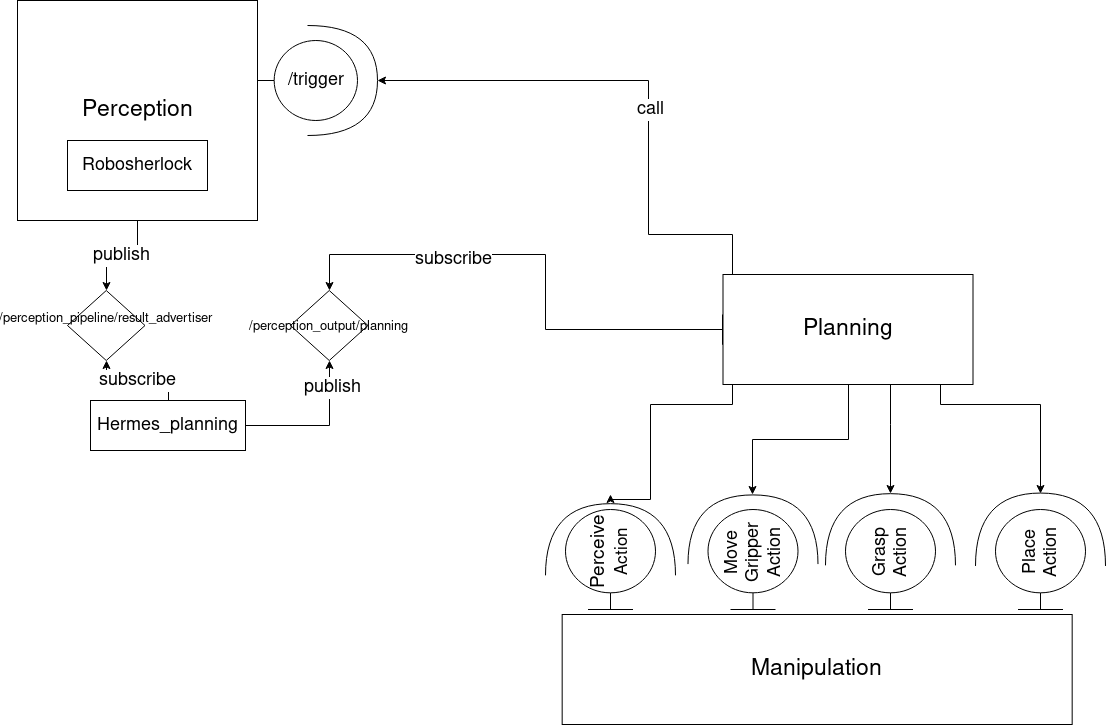
\includegraphics[width=0.85\textwidth]{pictures/diagramms/architecture.png}
			\caption{Architecture overview}
			\label{architecture}
		\end{figure}
		
		\section{Description}
			As seen in the diagram \(\ref{architecture}\), the component which each group was responsible for are visualized. The perception component consists mainly of the \textit{SuturoProcessManager} module which implements an process manager to execute the \textit{RoboSherlock} pipeline. The \textit{RoboSherlock} pipeline then handles the classification and annotation. The results are collected and converted by the \textit{SuturoProcessManager}.  The Knowledge component consists of the knowledge base which is a wrapped information storage (database) for the HSR, it handles position data as well as some logic for goal position determination. The Manipulation component is responsible for gripper movement, head/body movement and grasp/place operations. For this Manipulation is using \textit{Giskard}. The Navigation component is only used for moving the HSR and for collision avoidance during movement and uses the basic movement interface of the HSR. The Planning component uses cram to implement multi layered plans for executing the tasks. It is split in multiple levels cleanup \ref{clean} and grocery \ref{grocery} are the on highest level (execute level), these call functions from the mid level common functions \ref{comf} and the lowest level used for communication with other groups low level interfacing \ref{llif}.
			\begin{itemize}
				\item{\textbf{Cram}} \\
					 \textit{Cram} is a software toolbox for the design, the implementation, and the deployment of cognition-enabled autonomous robots
				\item{\textbf{Giskard}} \\
					\textit{Giskard} is a  framework for constraint based motion planning and execution.
				\item{\textbf{Julius}} \\
					\textit{Julius} is a continuous speech recognition software. It is capable of recognizing spoken sentence as-live. Julius' main strength is the fact, that it works on dictionaries. Dictionaries are a simple way for developers to adapt Julius to only recognize domain-specific sentences. Julius is not specifically created for ROS, but Toyota created a wrapper to allow the output of Julius to be published in ROS.
				\item{\textbf{KnowRob}} \\
				    \textit{KnowRob} is a framework created to combine different knowledge sources (such as knowledge about and provided by the robot, common sense, research etc.) and provide some reasoning methods to work with them. 
				\item{\textbf{Robosherlock}} \\
					\textit{RoboSherlock} is a common framework for cognitive perception, based on the principle of unstructured information management (UIM).
				\item{\textbf{Caffee}} \\
					\textit{Caffe} is a deep learning framework made with expression, speed, and modularity in mind. It is developed by Berkeley AI Research (BAIR) and by community contributors.

			\end{itemize}
	  		 

	\endgroup

\end{document}
